% !TEX root = ../Thesis.tex

\chapter{Sistemi Operativi}\label{cap:04}

Questo capitolo esplorerà le capacità offerte da Rust nel 
contesto della programmazione di sistema. In apertura verrà
fornita una panoramica sul linguaggio C, standard \textit{de facto}
nel contesto programmazione di sistema, con particolare attenzione alle 
 caratteristiche che lo rendono popolare in questo ambito.

Successivamente Rust verrà confrontato con C rispetto agli aspetti analizzati
, per valutare come Rust possa presentare un'alternativa valida sul piano teorico.

Nel capitolo~\ref{cap:05}, `\textit{<inserire nome>}', l'analisi verrà spostata sul piano pratico, 
esplorando progetti concreti, che mostrano le potenzialità di Rust nella programmazione di basso livello. \hfill
\vspace{20pt}\\
\noindent Nel contesto dei sistemi operativi, quali lo sviluppo di kernel, driver o componenti embedded i linguaggi tradizionalmente dominanti
 sono l'assembly e, con maggiore rilievo, C.

Nonostante l'esistenza di alternative come C++, Lisp, Forth o Bliss, la scelta spesso ricave esclusivamente
su C, come testimoniano le codebase dei sistemi operativi più popolari oggi giorno: Windows, MacOS, Linux e Android sono scritti quasi interamente nel linguaggio C.

Ma cosa rende C così popolare in questo ambito? Quali caratteristiche lo distinguono dalle alternative?

\section{C:\  motivazioni e caratteristiche}
C è un linguaggio di programmazione ampiamente utilizzato nella 
programmazione di sistema. Il linguaggio offre un livello
di astrazione molto vicino al codice macchina (o meglio, 
all'assembly), garantendo un certo grado di portabilità 
tra architetture differenti.

Si consideri, per esempio, quanto detto dal creatore del linguaggio:
\begin{center}
    \begin{minipage}{0.9\textwidth}
        \vspace{0.5em}
        \itshape "[C has] the power of the assembly language and the convenience of \ldots assembly language."

        \hfill --- Dennis Ritchie, creatore del linguaggio C, "Dennis Ritchie: The Shoulders Steve Jobs Stood On", *Wired*, 13 Oct 2011
        \vspace{0.4em}
    \end{minipage}
\end{center}
\noindent La popolarità di C in questo ambito è da attribuire a
diverse sue caratteristiche, alcune delle quali ben documentate\cite{c-system-programming-why}. 
Queste sono principalmente: compilazione, assenza di dipendenze 
runtime, gestione diretta della memoria, manipolazione 
a basso livello di bit e corrispondenza quasi diretta al codice macchina.

\subsection*{Compilazione}
C è un linguaggio compilato: il file eseguibile generato risulta 
molto efficiente, sotto l'aspetto della velocità d'esecuzione, 
rispetto a linguaggi interpretati. Questo lo rende preferibile nell'ambito di sviluppo
kernel, dove le prestazioni rappresentano un aspetto cruciale.

\subsection*{Assenza di dipendenze runtime}
C può essere impiegato per realizzare codice 
`\textit{bare metal}', eseguibile direttamente sull'hardware, 
senza il supporto di un sistema operativo. 

C non ha esigenze runtime significative: può funzionare anche senza un allocatore di memoria fornito dal 
sistema operativo\footnote{Un programma che non usufruisce della memoria 
dinamica non richiede un allocatore. Inoltre, nello sviluppo di un sistema 
operativo, è il programmatore che deve fornire il proprio sistema di allocazione.}. L'unica 
necessità minima è quella di un chiamante che invochi la funzione \textit{main}\footnote{In contesti a basso livello, quest a chiamata 
 può essere realizzata da codice assembly.}.

\subsection*{Accesso diretto alla memoria}
I puntatori C consentono l'accesso diretto a
indirizzi di memoria arbitrari, permettendo operazioni di lettura e 
scrittura dirette. 

Tale controllo sulla memoria è cruciale per lo sviluppo di un 
sistema operativo, dove è richiesto di gestire: tabelle delle pagine, dispositivi I/O mappati sulla memoria, controllori DMA e altri;

\subsection*{Manipolazione di bit}
Molte interazioni con l'hardware avvengono tramite operazioni bitwise, come riportato da \textit{Ada Computers}\cite{bitwise-operations}. 
Esempi comuni sono:
\begin{itemize}
    \item Operazioni di scrittura e lettura dei registri della CPU, come registri di flag di stato. Per esempio, in CPU x86 si trova il registro \textit{EFLAGS} che contiene una serie di bit di stato (\textit{overflow}, \textit{zero}, \textit{carry}, \textit{interrupt enable} e altri), il loro controllo di solito è fatto tramite l'applicazione di una maschera bitwise;
    \item Gestione delle periferiche mappate sulla memoria, tramite operazioni di abilitazione e disabilitazione dei singoli pin (e.g.\  registri \textit{GPIO});
    \item Il clock della CPU può essere gestito tramite operazioni bitwise.
\end{itemize}
Come riportato dal seguente articolo~\cite{bitwise-operations-c}, il linguaggio C supporta un ampio range di operazioni bitwise, offrendo i seguenti operatori: \textit{AND}, \textit{OR}, \textit{XOR}, \textit{SHL}, \textit{SHR}, \textit{NOT} e il complemento.

\subsection*{Somiglianza al codice macchina}
C mantiene una corrispondenza quasi \textit{1-to-1} in codice assembly. 
Questa trasparenza del linguaggio è fondamentale nello sviluppo di 
sistemi operativi, in quanto consente di comprendere l'effetto di ogni singola istruzione. 
C evita strutture dati complesse o astrazioni pesanti che potrebbero mascherare
il comportamento a basso livello del programma.\hfill
\vspace{30pt}\\
\noindent Tuttavia, uno dei punti di forza di C rappresenta anche una sua criticità. 
L'accesso diretto e non controllato della memoria, unito all'assenza di protezioni a runtime, rende semplice
commettere errori potenzialmente gravi come:
\begin{itemize}
    \item \textbf{Accessi non autorizzati alla memoria}: un programma che legge da un indirizzo di memoria arbitrario potrebbe inavvertitamente compromettere la privacy di un'altro processo; una scrittura accidentale potrebbe causare la corruzione della memoria, condivisa o utilizzata da un altro processo;
    \item \textbf{Saturazione della memoria}: un programma che alloca memoria senza controllo o limiti potrebbe esaurire la memoria disponibile. Se lo \textit{swapping} è disponibile, il sistema può degradare drasticamente le prestazioni; in caso non lo fosse, può verificarsi un crash.
\end{itemize}

\section{Rust contro C}
Nonostante Rust offra numerose astrazioni di alto livello\footnote{Rust offre delle astrazioni di alto livello definite \textit{zero cost}: feature quali \textit{iteratori}, \textit{generics}, \textit{smart pointers} e meccanismi di \textit{async/await} che vengono compilate in codice dalle prestazioni equivalenti alla controparte \textit{low-level} scritta a mano.}, è progettato come un linguaggio di basso livello, 
adatto alla programmazione di sistema.
Per comprendere le capacità di Rust nella programmazione di basso livello, verrà confrontato con il linguaggio C, sulla 
base delle caratteristiche che lo rendono favorevole nella programmazione di sistema.

La maggior parte delle informazioni riportate nella sezione è stata ricavata dalla documentazione ufficiale di Rust\cite{rust-book}.
\begin{itemize}
    \item \textbf{Compilazione} (Come C): Anche Rust è un linguaggio compilato. Il compilatore genera, in base alla piattaforma, un file direttamente eseguibile;
    \item \textbf{Dipendenze runtime} (Come C): Rust, per configurazione predefinita, ha dipendenze runtime minime (principalmente un allocatore di memoria). Tuttavia, come riportato in \textit{The Embedded Rust Book}\cite{rust-book-embedded}, tramite la direttiva \texttt{\#![no\_std]} è possibile escludere la libreria standard: in questa configurazione, l'unico requisito è un bootstrap che invochi la funzione \texttt{\_start} per fare iniziare l'esecuzione;
    \item \textbf{Accesso diretto alla memoria} (Come C): Tramite una parola chiave, \textit{unsafe}, Rust mette a disposizione cinque operazioni denominate \textit{superpoteri non sicuri}: tra queste si trovano anche la possibilità di dereferenziare un puntatore raw (come in C) e la possiblità di eseguire codice C o assembly;
    \item \textbf{Manipolazione di bit} (Come C): Rust offre lo stesso livello di manipolazione dei singoli bit di C, con un'unica differenza: le operazioni bitwise in Rust sono ben definite, evitando condizioni di \textit{Undefined Behaviour} tramite controlli statici sulle dimensione e tipi degli operandi;
    \item \textbf{Somiglianza al codice macchina} (Diverso da C): Rust generalmente offre astrazioni di alto livello, inoltre il compilatore può introdurre copie e spostamenti aggiuntivi per preservare le condizioni di ownership o inserire controlli su accessi e indici per gli \textit{slice}\footnote{Slice è un tipo primitivo in Rust. Sono un riferimento a una porzione contigua (in memoria) di elementi di una collezione. Non memorizzano dati esplicitamente, si tratta di una vista su dati esistenti.}. Tali comportamenti, pur aumentando la sicurezza, possono produrre un codice meno `trasparente' rispetto alla controparte C;\ 
\end{itemize}
Infine, a differenza di C, Rust garantisce l'integrità e la sicurezza della memoria già a tempo della compilazione, prevenendo 
errori comuni legati alla gestione della memoria grazie al \textit{modello di ownership}. In quanto i controlli effettuati
dal \textit{Borrow Checker} avvengono a tempo di compilazione non si hanno dipendenze o overhead introdotti a runtime.

\subsection*{Unsafe Rust}
Come già accennato, Rust mette a disposizione, tramite la parola chiave \textit{unsafe}, cinque operazioni principali. Gli sviluppatori
del progetto Rust si riferiscono a queste operazioni con l'espressione \textit{Unsafe Superpowers}:
\begin{itemize}
    \item Dereference di un puntatore raw;
    \item Invocazione di una funzione o metodo non sicuri;
    \item Accesso e modifica di una variabile mutabile e statica;
    \item Implementazione di un tratto non sicuro;
    \item Accesso ai campi di una \textit{union}.
\end{itemize}
Le espressioni \textit{Unsafe Rust} e \textit{Unsafe Superpowers} possono risultare fuorvianti: il \textit{Borrow Checker} esegue 
comunque controlli per garantire la validità delle reference. 

La parola chiave permette solamente di eseguire operazioni che, per definizione, sono considerate non sicure. 
Il compilatore non può controllarne la sicurezza e l'integrità durante la compilazione; all'interno di un blocco
 \textit{unsafe}, è il programmatore a diventare responsabile di garantire che gli accessi alla memoria
siano validi. \hfill
\vspace{12pt}\\
\noindent La \textit{best practice} riguardante i blocchi non sicuri prevede di ridurre il codice non sicuro il più possibile, utilizzandolo solo quando stretto necessario.
Inoltre, è preferito incapsulare il codice non sicuro all'interno di un'astrazione sicura, fornendo una API sicura per il suo utilizzo. \hfill

\subsection{Gestione delle risorse}

\subsection{Sicurezza della memoria}
In questa sottosezione verranno analizzati alcuni tra gli errori più comuni legati alla gestione della memoria,
mostrando esempi di codice scritti in C e confrontandoli, quando possibile, con le controparti in Rust.

Un aspetto interessante del modello di memoria di Rust è che alcuni errori non sono semplicemente rilevati
durante l'esecuzione, o a tempo di compilazione, ma sono strutturalmente impossibili da generare: non vi è modo di scrivere codice Rust che generi tali errori.
Come già accennato, il \textit{modello di ownership} guida la struttura di un programma in Rust: spinge il programmatore a
ragionare in termini di \textit{ownership} e \textit{lifetime}. Inoltre, l'allocazione della memoria dinamica è gestita tramite l'utilizzo
di \textit{smart pointers}, che forniscono un'astrazione sicura per la gestione della memoria dinamica.

% Unfreed memory
\subsubsection{Unfreed memory}
La \textit{unfreed memory} (memoria non liberata) rappresenta un errore comune durante la gestione della memoria dinamica tramite approccio manuale.
Si ha in quei contesti in cui aree di memoria vengono allocate, senza successiva deallocazione. Le aree di memoria interessate non
possono essere riutilizzate per allocazioni successive in quanto vengono considerate ancora utilizzate.

Si consideri il seguente esempio minimale C che genera un'errore di \textit{unfreed memory}:
\begin{lstlisting}[language=C, caption={Unfreed memory in C}, label={c:unfreed-memory}]
#include <stdlib.h>
int main(void) {
    void* mem = malloc(sizeof(int));
    return 0;
}
\end{lstlisting}
In Rust questo comportamento non si potrà mai realizzare, in quanto la deallocazione viene gestita implicitamente dal compilatore\footnote{Il compilatore inserisce chiamate alla funzione \textit{drop} in corrispondenza della fine di uno scope. Questo è realizzabile in quanto il \textit{Borrow Checker} controlla le relazioni di \textit{ownership} e \textit{borrowing} per determinare chi sia responsabile della deallocazione, ovvero su quali variabili invocare \textit{drop}.}. \hfill

\noindent Si consideri un programma in Rust che, per quanto possibile, replica il comportamento del listato~\ref{c:unfreed-memory}:
\begin{lstlisting}[language=Rust, caption={Unfreed memory in Rust}, label={rust:unfreed-memory}]
fn main() {
    let mem = Box::<u32>::new(0);
}
\end{lstlisting}
Nel listato~\ref{c:unfreed-memory} viene allocata memoria nella heap sufficiente a contenere un intero, successivamente 
il programma termina senza liberarla\footnote{In realtà l'allocazione avviene nello spazio di memoria virtuale del processo; a termine dell'esecuzione, il sistema operativo recupera tutte le risorse allocate dal processo.}. 
Il programma viene compilato ed eseguito correttamente, 
nonostante la presenza di questo errore. 
Tuttavia, tale memoria risulta inaccessibile per ulteriori allocazioni da parte del processo durante la sua esecuzione.\hfill
\vspace{10pt}\\
\noindent Il listato~\ref{rust:unfreed-memory} rappresenta il codice Rust più vicino possibile a 
quello riportato nel listato~\ref{c:unfreed-memory}. La differenza principale è che la memoria viene deallocata automaticamente: 
al termine dello scope della funzione \texttt{main}, la variabile \texttt{mem} viene eliminata e la relativa 
memoria deallocata. 

Di conseguenza, l'errore di \textit{unfreed memory} non può manifestarsi, in quanto la deallocazione avviene in maniera 
trasparente agli occhi del programmatore. 


% Double free
\subsubsection{Double free}
La \textit{double free} (doppia liberazione) è un'errore di gestione della memoria che si verifica quando la stessa area di memoria viene deallocata
più di una volta. Ciò può causare la corruzione della memoria heap, con conseguente comportamento indefinito o crash del programma.

Nel linguaggio C, questo si verifica invocando la funzione \texttt{free} sullo stesso puntatore più volte, come mostrato 
nel seguente esempio:
\begin{samepage}
\begin{lstlisting}[language=C, caption={Double free in C}, label={c:double-free}]
#include <stdlib.h>
int main(void) {
    void* ptr = malloc(sizeof(int));
    free(ptr);
    free(ptr);
    return 0;
}
\end{lstlisting}
\end{samepage}
Si consideri invece il seguente programma Rust che tenta di replicare lo stesso comportamento del listato~\ref{c:double-free}:
\begin{lstlisting}[language=Rust, caption={Double free in Rust}, label={rust:double-free}]
fn main() {
    let mem = Box::<u32>::new(0);
    std::mem::drop(mem);
    std::mem::drop(mem);
}
\end{lstlisting}
Nel listato~\ref{c:double-free} la memoria puntata da \texttt{ptr} viene deallocata due volte.
In fase di esecuzione questo può portare a un crash del programma, come mostrato nell'immagine~\ref{c:double-free-exec}.

Tuttavia, lo standard C non definisce un comportamento specifico da adottare in questo contesto, causando 
\textit{undefined behaviour} nella pratica\footnote{In ambiente Linux con \texttt{glibc}, viene rilevato l'errore causando
 la stampa di un messaggio e l'interruzione dell'esecuzione. In ambienti Windows, l'errore può passare inosservato o causare un crash silenzioso.}.

Per quanto riguarda Rust, è possibile considerare due scenari: 
\begin{itemize}
    \item Il listato~\ref{rust:unfreed-memory} rappresenta il comportamento idiomatico di Rust: la memoria viene deallocata automaticamente alla fine di uno \textit{scope}, senza necessità di interventi manuali;
    \item Nel listato~\ref{rust:double-free}, invece, si tenta di deallocare esplicitamente la memoria con due chiamate consecutive a \texttt{std::mem::drop}\footnote{Questa funzione assume \textit{ownership} del valore fornito, causandone la deallocazione una volta raggiunta la fine della funzione.}. Tuttavia, la funzione \texttt{drop} prende possesso del valore, rendendo la reference originale, e di conseguenza la seconda chiamata, invalida. Il compilatore si accorge della violazione della terza regola di \textit{borrowing} (\textit{Tutte le reference devono essere valide}), impedendo la compilazione e generando l'errore riportato nell'immagine~\ref{rust:double-free-compile}.
\end{itemize}
\begin{figure}[htbp]
\begin{center}
    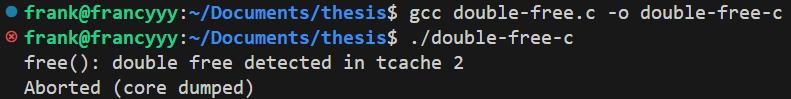
\includegraphics[width=.8\textwidth]{double-free-c-exec}
    \caption{\textit{Double free} in C}\label{c:double-free-exec}
    \end{center}
\end{figure}
\begin{figure}[htbp]
\begin{center}
    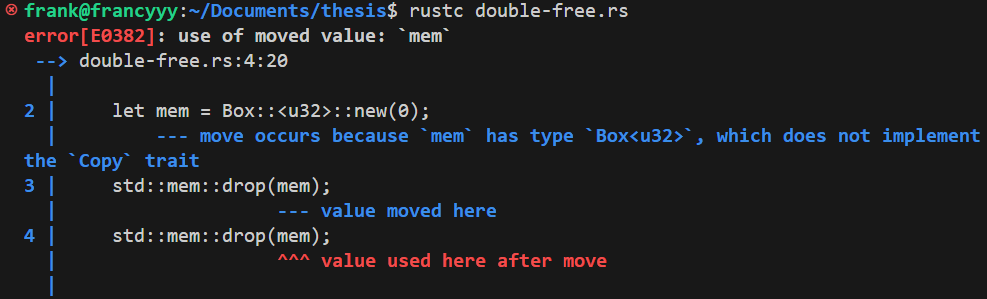
\includegraphics[width=.8\textwidth]{double-free-rust-compile}
    \caption{Tentativo di \textit{double free} in Rust}\label{rust:double-free-compile}
    \end{center}
\end{figure}

% Dangling pointer
\subsubsection{Dangling pointers}
Un \textit{dangling pointer} (puntatore pendente) è un puntatore che riferisce a una locazione di memoria non più valida o che è stata liberata. 
Generalmente si presenta quando un'area di memoria viene deallocata, ma gli eventuali puntatori che la referenziavano non vengono aggiornati.

Si consideri il seguente esempio C che genera un \textit{dangling pointer}\footnote{La presenza di uno scope interno non è funzionale all'esempio, ma non ne modifica nemmeno il risultato. È presente per garantire somiglianza strutturale con l'esempio Rust successivo.}:
\begin{lstlisting}[language=C, caption={Dangling pointer in C}, label={c:dangling-pointer}]
int main(void) {
    int* ptr;
    {
        int* val = malloc(sizeof(int));
        *val = 30;
        ptr = val;
        free(val);
    }
}
\end{lstlisting}
Nel listato~\ref{c:dangling-pointer}, viene allocata memoria sufficiente per un intero e il suo indirizzo è memorizzato 
sia in \texttt{val} che in \texttt{ptr}. La memoria viene successivamente deallocata invocando la funzione \texttt{free} sul puntatore \texttt{val}.
Tuttavia, il puntatore \texttt{ptr} non viene aggiornato, continuando a riferire alla stessa area di memoria, ormai non più valida.

È importante osservare che la sola esistenza un un \textit{dangling pointer} non causa un errore immediato.
Il comportamento indefinito si manifesta solo quando si tenta di derefenziare tale puntatore, cercando di leggere o scrivere nella memoria a cui fa riferimento. \hfill
\vspace{12pt}\\
\noindent A dimostrazione di ciò, si consideri che Rust permette la creazione di una \textit{dangling reference}, a patto che non venga utilizzata.
Il seguente esempio mostra questa possibilità:
\begin{lstlisting}[language=Rust, caption={Dangling reference in Rust}, label={rust:dangling-pointer}]
fn main() {
    let _ref: &u32;
    {
        let val = Box::<u32>::new(30);
        _ref = &*val;
    }
}
\end{lstlisting}
Il listato~\ref{rust:dangling-pointer} tenta di replicare, per quanto possibile, il comportamento descritto nel listato~\ref{c:dangling-pointer}:
alla variabile \texttt{\_ref} viene assegnato un riferimento a \texttt{val}, allocata dinamicamente in uno scope interno. All'uscita 
da tale scope, \texttt{val} viene deallocato, lasciando \texttt{\_ref} con un riferimento non valido. 

Nonostante ciò, il compilatore non genera alcun errore.
Questo comportamento è giustificato dal fatto che la reference non è mai utilizzata\footnote{Il \textit{Borrow Checker} lavora in maniera \textit{lazy}: non verifica 
le condizioni di \textit{borrowing} e \textit{lifetime} di una reference fino a che non viene utilizzata.} e, di conseguenza, il \textit{Borrow Checker} non rileva alcuna
 violazione delle regole di \textit{borrowing}.

% Access after free
\subsubsection{Access after free}
Sebbene la sola presenza di un \textit{dangling pointer} non causi immediatamente problemi, essa rappresenta una condizione necessaria 
per un errore più grave: la \textit{access after free} (accesso post-liberazione).
Questo errore si verifica quando si tenta di accedere a memoria precedentemente deallocata, dereferenziando un \textit{dangling pointer}. 

A seconda del tipo
di accesso, si possono avere conseguenze differenti:
\begin{itemize}
    \item \textbf{Lettura}: può causare il recupero di dati non validi o incoerenti, eventualmente sovrascritti da allocazioni successive;
    \item \textbf{Scrittura}: può compromettere l'integrità della memoria, causando comportamenti indefiniti o crash del programma.
\end{itemize}
Si consideri il seguente esempio C che, estendendo il listato~\ref{c:dangling-pointer}, genera un errore di \textit{access after free}:
\begin{lstlisting}[language=C, caption={Access after free in C}, label={c:access-after-free}]
#include <stdlib.h>
#include <stdio.h>
int main(void) {
    int* ptr;
    {
        int* val = malloc(sizeof(int));
        *val = 30;
        ptr = val;
        free(val);
    }
    printf("%d\n", *ptr);
}
\end{lstlisting}
Nel listato~\ref{c:access-after-free} si tenta di dereferenziare il puntatore \texttt{ptr} dopo che la memoria a cui faceva riferimento è stata deallocata.
In questo caso, l'accesso avviene per effettuare un'operazione di lettura, che rappresenta una forma
 meno distruttiva rispetto a una scrittura, ma che resta comunque pericolosa:
i dati letti potrebbero essere non validi o casuali, in quanto la memoria potrebbe essere stata sovrascritta da allocazioni successive.
 
Questo comportamento rappresenta un esempio di \textit{undefined behaviour}, come illustrato
dall'immagine~\ref{c:access-after-free-exec}. \hfill
\vspace{12pt}\\
\noindent Per osservare come Rust gestisce questa problematica, si consideri il seguente esempio, il quale estende il listato~\ref{rust:dangling-pointer}:
\begin{lstlisting}[language=Rust, caption={Tentativo di access after free in Rust}, label={rust:access-after-free}]
fn main() {
    let _ref: &u32;
    {
        let val = Box::<u32>::new(30);
        _ref = &*val;
    }
    println!("{}", _ref);
}
\end{lstlisting}
Il listato~\ref{rust:dangling-pointer} tenta di replicare il comportamento del listato~\ref{c:access-after-free}, cercando 
di accedere a una reference pendente per un'operazione di lettura.

Tuttavia, in questo caso viene generato un errore di compilazione, come mostrato nell'immagine~\ref{rust:access-after-free-compile}.
Il \textit{Borrow Checker} rileva che \texttt{\_ref} viene utilizzata successivamente alla deallocazione di \texttt{val}, rappresentando una violazione 
delle regole di \textit{borrowing} e, di conseguenza, impedisce la compilazione.
\begin{figure}[htbp]
\begin{center}
    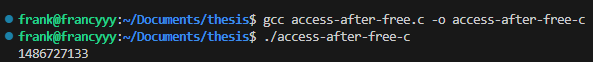
\includegraphics[width=.8\textwidth]{access-after-free-c-exec}
    \caption{\textit{Access after free} in C}\label{c:access-after-free-exec}
    \end{center}
\end{figure}
\begin{figure}[htbp]
\begin{center}
    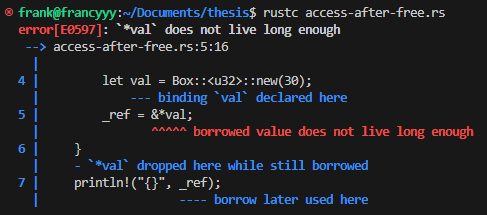
\includegraphics[width=.8\textwidth]{access-after-free-rust-compile}
    \caption{Tentativo di \textit{access after free} in Rust}\label{rust:access-after-free-compile}
    \end{center}
\end{figure}

% Buffer Overflow e Overread
\subsubsection{Access out of bounds: buffer overflow e overread}
L' \textit{access out of bounds} è un errore comune associatio alla gestione manuale della memoria dinamica.
Si verifica quando si tenta di accedere a una porzione di memoria al di fuori dei limiti dell'area effettivamente allocata.

In base al tipo di accesso si distingue in due varianti: nel caso di una lettura si parla di \textit{buffer overread} 
(lettura oltre i limiti) mentre, nel caso di una scrittura, di \textit{buffer overflow} (sovraccarico o sovrascrittura del buffer).

\paragraph{Buffer overflow}
Si consideri il seguente esempio C che genera un errore di \textit{buffer overflow}:
\begin{lstlisting}[language=C, caption={Buffer overflow in C}, label={c:buffer-overflow}]
#include <stdlib.h>
#include <stdio.h>
int main(void) {
    int* vec = malloc(sizeof(int) * 3);
    printf("Allocato un vettore di 3 interi, indici validi: 0, 1, 2\n");
    for(int i = 0; i <= 3; i++) {
        printf("Memorizzando %d all'indice %d\n", i * 10, i);
        vec[i] = i * 10;
    }
    free(vec);
    printf("Terminata la memorizzazione!\n");
    return 0;
}
\end{lstlisting}
Nel listato~\ref{c:buffer-overflow} viene allocata memoria suffiente per un vettore di tre interi, ma successivamente vengono
inizializzati quattro elementi, dall'indice \texttt{0} fino a \texttt{3}.
In questo caso il programma termina senza errori, viene anche eseguita la stampa finale, come mostrato dall'immagine~\ref{c:buffer-overflow-exec}. 

Nonostante ciò, questo comportamento non può essere considerato una garanzia in quanto, generalmente, la conseguenza di un \textit{buffer overflow} è un \textit{undefined behaviour}: 
non è possibile determinare a priori cosa contenga la memoria oltre
il limite dell'allocazione o per cosa venga utilizzata\footnote{In generale un \textit{buffer overflow} avviene all'interno dello spazio
di indirizzamento virtuale di un processo. In questo caso, la memoria potenzialmente corrotta sarebbe
 del processo stesso. Tuttavia, nel caso in cui l'indirizzo di riferimento
 fosse al di fuori dello spazio di indirizzamento virtuale del processo verrebbe generato un'errore runtime di tipo \textit{segmentation fault}, 
 causando l'immediato crash del programma.}. \hfill
\vspace{10pt}\\
\noindent Per comprendere come Rust gestisca questo errore, si consideri il seguente esempio:
\begin{lstlisting}[language=Rust, caption={Buffer overflow in Rust}, label={rust:buffer-overflow}]
fn main() {
    let mut vec: Vec<u32> = vec![0; 3];
    println!("Allocato un vettore di 3 interi, indici validi: 0, 1, 2");
    for i in 0u32..=3u32 {    
        println!("Memorizzando {} all'indice {}", i * 10, i);
        vec[i as usize] = i * 10;
    }
    println!("Terminata la memorizzazione!");
}
\end{lstlisting}
Il listato~\ref{rust:buffer-overflow} tenta di replicare il comportamento del listato~\ref{c:buffer-overflow}, 
allocando un vettore di tre interi e successivamente cercando di inizializzarne quattro. 
In questo caso la compilazione va a buon fine, ma la stampa finale non avviene: il programma genera un \textit{panic} durante l'esecuzione. Questo avviene
durante l'accesso all'indice \texttt{3}, come mostrato nell'immagine~\ref{rust:buffer-overflow-exec}.

Questo comportamento è dovuto al fatto che il compilatore inserisce controlli di validità sugli indici, i quali vengono eseguiti a runtime.\footnote{Infatti, il compilatore non può sapere a tempo di compilazione quali sarnno gli indice che verranno utilizzati per accedere a un vettore, quindi si limita a inserire controlli sulla loro validità prima degli accessi effettivi.}
\begin{figure}[htbp]
\begin{center}
    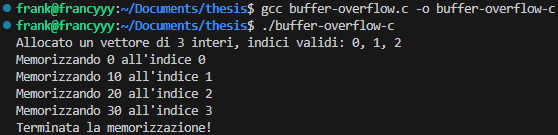
\includegraphics[width=.8\textwidth]{c-buffer-overflow-exec}
    \caption{\textit{Buffer overflow} in C}\label{c:buffer-overflow-exec}
    \end{center}
\end{figure}
\begin{figure}[htbp]
\begin{center}
    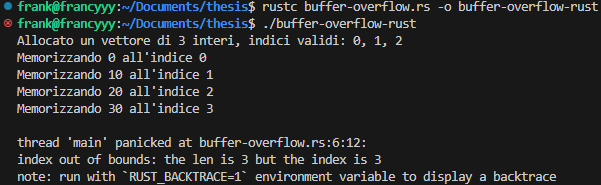
\includegraphics[width=.8\textwidth]{rust-buffer-overflow-exec}
    \caption{\textit{Buffer overflow} in Rust}\label{rust:buffer-overflow-exec}
    \end{center}
\end{figure}


\paragraph{Buffer overread}
Si consideri il seguente esempio C che genera un errore di \textit{buffer overread}:
\begin{lstlisting}[language=C, caption={Buffer overread in C}, label={c:buffer-overread}]
#include <stdlib.h>
#include <stdio.h>
int main(void) {
    int* vec = malloc(sizeof(int) * 3);
    for(int i = 0; i < 3; i++) vec[i] = i * 10;
    printf("Contenuto del vettore:\n");
    for(int i = 0; i < 10; i++)
        printf("Indice: %d -> Valore: %d\n", i, vec[i]);
    free(vec);
    return 0;
}
\end{lstlisting}
Nel listato~\ref{c:buffer-overread} viene allocata memoria per un vettore di tre interi, i quali vengono correttamente inizializzati e, successivamente,
si tenta di leggere dieci elementi dal vettore.
In questo caso il programma termina senza errori, stampando effettivamente dieci elementi, come mostrato dall'immagine~\ref{c:buffer-overread-exec}. 

Come quanto detto per l'errore di \textit{buffer overflow}, generalmente la conseguenza è un \textit{undefined behaviour}: 
non è possibile determinare a priori cosa contenga la memoria (oltre
il limite dell'allocazione) che viene letta\footnote{Vangono le stesse considerazioni fatte per il \textit{buffer overflow}: un'accesso a un indirizzo
che eccede lo spazio di indirizzi virtuali del processo genera un errore runtime di tipo \textit{segmentation fault}, causando l'immediato crash del programma}.\hfill
\vspace{10pt}\\
\noindent Rust gestisce questo errore in maniera analoga al \textit{buffer overflow}. Si consideri a dimostrazione di ciò il seguente esempio:
\begin{lstlisting}[language=Rust, caption={Buffer overread in Rust}, label={rust:buffer-overread}]
fn main() {
    fn main() {
    let vec: Vec<u32> = vec![0, 10, 20];
    println!("Contenuto del vettore:");
    for i in 0..10 {
        println!("Indice: {} -> Valore: {}", i, vec[i]);
    }
}
}
\end{lstlisting}
Il listato~\ref{rust:buffer-overread} tenta di replicare il comportamento del listato~\ref{c:buffer-overread}, 
allocando un vettore di tre interi e successivamente cercando di leggerne dieci. 

Anche in questo caso la compilazione termina correttamente ma, durante l'esecuzione, in particolare durante l'accesso al quarto elemento, viene generato
un \textit{panic}. 

Questo comportamento può essere osservato nell'immagine~\ref{rust:buffer-overread-exec}.
\begin{figure}[htbp]
\begin{center}
    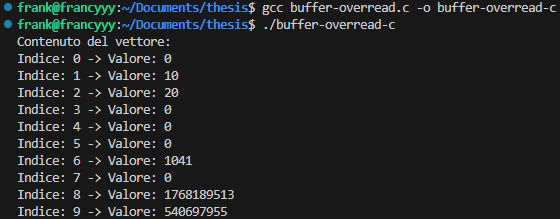
\includegraphics[width=.8\textwidth]{c-buffer-overread-exec}
    \caption{\textit{Buffer overread} in C}\label{c:buffer-overread-exec}
    \end{center}
\end{figure}
\begin{figure}[htbp]
\begin{center}
    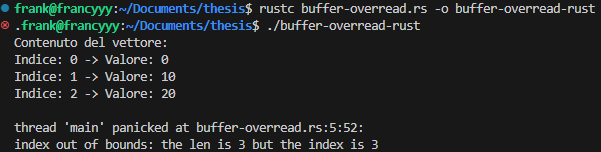
\includegraphics[width=.8\textwidth]{rust-buffer-overread-exec}
    \caption{\textit{Buffer overread} in Rust}\label{rust:buffer-overread-exec}
    \end{center}
\end{figure}

% Unitialized memory access
\subsubsection{Unitialized memory access} 
La \textit{unitialized memory access} (accesso a memoria non inizializzata) è un errore che si presenta
 quando si tenta di leggere da un'area di memoria che non è stata 
 inizializzata. Questo può portare a comportamenti imprevedibili, in quanto 
 i dati letti potrebbero essere casuali e potenzialmente 
 residui da allocazioni precedenti.

Nel linguaggio C, questo errore si presenta tipicamente quando viene 
allocata memoria tramite la funzione \texttt{malloc} e successivamente si tenta di 
accedervi senza previa inizializzazione.

Si consideri il seguente esempio C che genera un errore di questo tipo:
\begin{lstlisting}[language=C, caption={Uninitialized memory access in C}, label={c:uninitialized-memory-access}]
#include <stdlib.h>
#include <stdio.h>
int main(void) {
    int* ptr = malloc(sizeof(int));
    printf("%d\n", *ptr);
    free(ptr);
    return 0;
}
\end{lstlisting}
Nel listato~\ref{c:uninitialized-memory-access} viene allocata memoria sufficiente a contenere un intero e, senza inizializzarne il contenuto,
viene tentato un accesso in lettura. 
Il risultato è un comportamento indefinito: il valore letto potrebbe variare in base all'ambiente di esecuzione e tra esecuzioni, senza garanzia di coerenza.

È possibile osservare un caso particolare, in cui l'accesso può sembrare produrre un risultato coerente, come mostrato nell'immagine~\ref{c:uninitialized-memory-access-exec}\footnote{L'esecuzione è avvenuta su Ubuntu LTS 24.04 con \texttt{glibc}. In questo contesto è possibile che \texttt{malloc} azzeri la memoria allocata, prima di restituirne l'indirizzo, ma non è un comportamento garantito dallo standard C.}.
Tuttavia, questa apparente stabilità non può essere considerata una garanzia, in quanto vi sono più fattori che possono influenzare il valore letto:
\begin{itemize}
    \item Implementazioni specifiche dell'allocatore di memoria, che possono inizializzare la memoria allocata a zero o a un valore casuale;
    \item La posizione in memoria scelta dall'allocatore per il puntatore;
    \item Eventuali valori residui da allocazioni precedenti;
    \item La mappatura tra pagine virtuali e fisiche da parte del sistema operativo.
\end{itemize}
A conferma dell'inaffidabilità, si consideri il seguente esempio, che estende il listato~\ref{c:uninitialized-memory-access}: 
\begin{lstlisting}[language=C, caption={Uninitialized memory access in C}, label={c:uninitialized-memory-access-2}]
#include <stdlib.h>
#include <stdio.h>
int main(void) {
    int* ptr = malloc(sizeof(int));
    free(ptr);
    ptr = malloc(sizeof(int));
    printf("%d\n", *ptr);
    free(ptr);
    return 0;
}
\end{lstlisting}
Il listato~\ref{c:uninitialized-memory-access-2} mostra come eseguire una \texttt{free} prima della \texttt{malloc} successiva può lasciare residui nella memoria. 
Di conseguenza il valore letto, questa volta, è diverso da zero, come si può osservare dall'immagine~\ref{c:uninitialized-memory-access-exec-2}\footnote{Anche in questo caso, si tratta di un comportamento specifico del sistema e non garantito dallo standard}.
\begin{figure}[htbp]
\begin{center}
    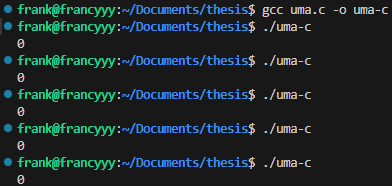
\includegraphics[width=.6\textwidth]{c-uninitialized-memory-access-exec}
    \caption{\textit{Uninitialized memory access} in C}\label{c:uninitialized-memory-access-exec}
    \end{center}
\end{figure}
Rust previene questa problematica in maniera strutturale, non permettendo allocazioni dinamiche senza inizializzazione grazie all'utilizzo di \texttt{smart pointers}, i quali prevedono un'inizializzazione obbligatoria.

In Rust infatti, le principali primitive per l'allocazione dinamica richiedono sempre l'inizializzazione dei valori:
\begin{itemize}
    \item \texttt{Box}: \textit{smart pointer} impiegato per allocare un singolo valore nella heap. L'unico modo per crearne uno è tramite \texttt{Box::new}, che richiede un valore per l'inizializzazione. In \textit{safe} Rust, non esiste un costrutto equivalente alla \texttt{malloc} in C;\ 
    \item \texttt{Vec}: \textit{smart pointer} utilizzato per una collezione dinamica di valori in heap. Anche se può essere creato vuoto (\texttt{Vec::new}), ogni accesso è verificato a runtime per evitare accessi oltre i limiti. In caso di violazioni viene generato un \texttt{panic}, terminando l'esecuzione, come è osservabile nell'immagine [mettere sopra];
\end{itemize}
Di conseguenza, non è possibile sviluppare codice Rust che acceda a memoria non inizializzata senza ricorrere alla parola chiave \texttt{unsafe}\footnote{Rust consente l'accesso a memoria potenzialmente non inizializzata, ma soltanto all'interno di blocchi \textit{unsafe}. Un esempio è la funzione \texttt{std::mem::MaybeUninit}, ma meccanismi come questo sono riservati a casi particolari, in cui le garanzie di sicurezza devono essere gestite manualmente dal programmatore.}.
\begin{figure}[htbp]
\begin{center}
    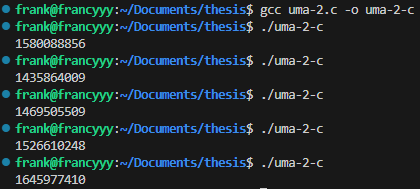
\includegraphics[width=.6\textwidth]{c-uninitialized-memory-access-exec-2}
    \caption{\textit{Uninitialized memory access} in C con previa \texttt{free}}\label{c:uninitialized-memory-access-exec-2}
    \end{center}
\end{figure}

\subsubsection{Sicurezza della memoria: conclusioni}
In conclusione, sotto l'aspetto della sicurezza della memoria, Rust si distingue da C garantendo un comportamento sicuro e deterministico, prevenendo
alcuni errori durante la compilazione e rilevandone altri a runtime. In C, d'altra parte, tali errori possono passare inosservati, causando
\textit{undefined behaviour} o crash del programma.

\subsection{Prestazioni}

\subsection{Complessità del codice}
Una critica comune nei confronti di Rust, specialmente da coloro che provengono da C, è la maggiore complessità e verbosità del linguaggio.
Generalmente, la sintassi di C è considerata più semplice e minimale, principalmente per la sua natura a basso livello, la mancanza di astrazioni
complesse e la presenza di un numero limitato di costrutti.

Al contrario in Rust, dovendo gestire attentamente le relazioni di \textit{ownership}, \textit{borrowing} e \textit{lifetime}, il codice può risultare più complesso; 
questi non sono gli unici aspetti che contribuiscono a questa percezione: gestione degli errori, controllo del flusso, supporto a \textit{generics} e \textit{macro} sono
tutti elementi che possono rendere il linguaggio più verboso e complesso rispetto a C.

\paragraph{Annotazioni di lifetime}

\paragraph{Generics}
Le espressioni \textit{generics} o \textit{generic programming} indicano un meccanismo di astrazione che consente di sviluppare codice indipendente da un tipo di dato specifico.
Il tipo viene fornito come argomento, generalmente in fase di compilazione, consentendo il riuso del codice con diversi tipi di dato. \hfill
\vspace{8pt}\\
\noindent Il linguaggio C non supporta nativamente lo sviluppo di codice parametrico, in quanto comporterebbe un livello di astrazione superiore rispetto alla
semplicità a cui il linguaggio aspira. Nonostante ciò, è possibile emulare un comportamento simile, principalmente tramite l'uso di puntatori \texttt{void*}, i quali possono riferirsi a valori di qualunche tipo.
Questo meccanismo, per quanto flessibile, richiede controlli rigorosi da parte del programmatore: 
\begin{itemize}
    \item un puntatore \texttt{void*} non memorizza informazioni sulla dimensione del valore puntato, rendendo necessaria la conoscenza esplicita del tipo (solitamente memorizzandone la dimensione);
    \item le operazioni di accesso, sia in lettura che scrittura, devono essere effettuate tramite funzioni delicate come \texttt{memcpy}, in quanto non è possibile dereferenziare direttamente un puntatore \texttt{void*}.
\end{itemize}
Il listato~\ref{c:generics} riporta un'estratto da un'implementazione in C di un nodo di una lista generica. L'implementazione completa è disponibile sulla piattaforma Github\footnote{Disponibile nel repository, \texttt{C-data-structures}, personale del candidato, seguendo il percorso: \texttt{src/linear/}. Alcuni commenti sono stati rimossi o spostati per ragioni di spazio.}.
\begin{lstlisting}[language=C, float, caption={Programmazione generica in C}, label={c:generics}]
typedef struct clinkedlist {
	node* tail;
	size_t element_count; /* Number of elements present in the list */
	size_t element_size; /* Size of the elements stored in the list */
} clinkedlist;

typedef struct node {
	void* ptr; /* Pointer to the memory location that stores the node's value */
	node* next; /* Pointer to the next node */
} node;

node* node_create(void* value, size_t value_size) {

	node* n = NULL;
	if (value_size <= SIZE_MAX) {

		n = (node*)malloc(sizeof(node));
		if (n) {

			n->ptr = malloc(value_size);
			if (n->ptr) {

				memcpy(n->ptr, value, value_size);
				n->next = NULL;
			}
			else {
				free(n);
				n = NULL;
			}
		}
	}
	return n;
}
\end{lstlisting}
Nell'implementazione di riferimento sono state adottate alcune strategie per cercare di prevenire errori legati alla gestione manuale dei tipi e della memoria:
\begin{itemize}
    \item \textbf{Tipo opaco}: la struttura dati è definita solo nel file sorgente, mentre l'header contiene solo una dichiarazione incompleta (\textit{opaque type}). Questo impedisce l'accesso diretto ai campi, tra cui \texttt{element\_size} di \texttt{clinkedlist}, la cui integrità è fondamentale per il corretto funzionamento della struttura;
    \item \textbf{Incapsulamento parziale}: la manipolazione della struttura è possibile solo tramite le funzioni fornite, obbligando l'utente a seguire un percorso logico e controllato per l'inserimento, la rimozione e la lettura dei dati. Questo permette l'introduzione di controlli interni riguardanti la validità e la coerenza dei dati. 
\end{itemize}
Nonostante queste precauzioni, il modello rimane fragile, per via della natura del linguaggio: l'utilizzo di \texttt{void*} permette la memorizzazione di qualsiasi valore, tra cui anche, altri puntatori; tuttavia, una eccessiva stratificazione di indirezione (i.e.\  puntatori a puntatori) può compromettere
la corretta deallocazione della memoria. \hfill
\vspace{15pt} \\
\noindent Rust adotta un approccio diverso, supportando la programmazione generica tramite le cosiddette \textit{zero-cost abstractions}\footnote{Si tratta di meccanismi e implementazioni astratti che non introducono overhead in fase di esecuzione rispetto al codice esplicito (concreto) equivalente.}.
Durante la fase di compilazione, il compilatore applica un processo detto \textit{monomorfizzazione}, trasformando ogni utilizzo di una funzione o una struttura
generica in una versione specifica per il tipo utilizzato.\hfill 
%Rust consente inoltre di specificare vincoli sui tipi generici (\textit{trait bounds}), tramite \texttt{impl Trait} e \texttt{where}. Questi meccanismi sono equivalenti, rispettivamente, a \texttt{implements Interface} e \texttt{<T extends \ldots>} di Java. \hfill
\vspace{8pt}\\
\noindent Per ottenere un confronto sulla complessità del codice, viene riportato, nel listato~\ref{rust:generics}, l'implementazione in Rust del listato~\ref{c:generics}: 
il supporto alla programmazione generica di Rust permette di definire strutture dati e funzioni generiche con codice sicuro e conciso.
\begin{lstlisting}[language=C, float, caption={Programmazione generica in Rust}, label={rust:generics}]
struct Clinkedlist<T> {
	tail: Option<Box<Node<T>>>,
	element_count: usize
}

struct Node<T> {
    value: T,
    next: Option<Box<Node<T>>>
}

impl<T> Node<T> {
    fn new(value: T) -> Node<T> {
        Node {
            value,
            next: None
        }
    }
}
\end{lstlisting}

L'implementazione risulta più semplice rispetto alla controparte C:\ non è necessario gestire manualmente la dimensione dei valori o gli accessi diretti alla memoria.
A tal proposito, si consideri che \texttt{Node::<T>::new()} del listato~\ref{rust:generics} è l'equivalente di \texttt{node\_create} del listato~\ref{c:generics}.

\paragraph{Controllo del flusso}

\paragraph{Gestione degli errori}
I due linguaggi si distinguono per i meccanismi impiegati per la gestione degli errori.
In C, tipicamente, tale gestione è opzionale: il linguaggio non impone alcun controllo esplicito, lasciando la responsabilità al programmatore.
Il meccanismo maggiormente diffuso per segnalare errori è basato sul valore di ritorno, tipicamente interi, da parte delle funzioni, secondo
convenzioni informali e non uniformi\footnote{Lo standard C non definisce una convenzione uniforme sugli interi da utilizzare come codice di errore. Alcune funzioni
utilizzano 0 per indicare successo e ogni altro valore viene interpretato come fallimento. Per questo motivo, è sempre opportuno controllare la documentazione di una funzione,
per determinare come interpretare l'esito: alcune funzioni potrebbero intepretare ogni valore non negativo con successo, come altre potrebbero utilizzare 0 per fallimento.}.

L'assenza di vincoli espliciti sul controllo dell'esito rende facile, e comune, la mancata verifica di errori. 
Questo tuttavia può portare a comportamenti indefiniti, principalmente dovuti all'elaborazione di dati non validi, derivanti da
chiamate a funzioni fallite, il cui risultato viene interpretato come se fosse corretto. \hfill
\vspace{9pt}\\
\noindent Come riportato dalla documentazione ufficiale\cite{rust-book}, Rust distingue tra due classi di errori, 
\textit{recuperabili} e \textit{irrecuperabili}, fornendo meccanismi distinti per la loro gestione.

Gli errori \textit{irrecuperabili} rappresentano situazioni dalle quali non è sicuro proseguire con l'esecuzione del programma, come l'accesso oltre i limiti di un array o 
il tentativo di dereferenziare un valore \texttt{None}\footnote{Rust utilizza l'enumerazione \texttt{Option<T>} per rappresentare un valore opzionale: \texttt{Some(T)} rappresenta la presenza di un valore, di tipo \texttt{T}, mentre \texttt{None} rapprenta l'assenza di un valore valido}. 
Rust gestisce questo tipo di errore tramite \textit{panic}, i quali causano l'immediata interruzione del programma e rilasciano correttamente
tutte le risorse allocate dal processo.

Al contrario, gli errori \textit{recuperabili} rappresentano situazioni meno gravi, per le quali è possibile definire una logica di gestione, senza necessità di interruzione: per esempio, il tentativo di apertura di un file inesistente potrebbe essere gestito creando il file, invece di terminare l'esecuzione.
Per la gestione di questo tipo di errore, Rust offre l'enumerazione \texttt{Result<T, E>}, in cui \texttt{T} ed \texttt{E} sono tipi generici:
\begin{itemize}
    \item \texttt{\textbf{Ok(T)}}: rappresenta la variante di Result che indica successo, contenente il valore, di tipo \texttt{T}, restituito;
    \item \texttt{\textbf{Err(E)}}: è la variante di Result che indica un fallimento, contenente un valore descrittivo dell'errore, di tipo \texttt{E}, generato.
\end{itemize}
A differenza del C, la gestione esplicita degli errori è obbligatoria in Rust: gli errori irrecuperabili vengono gestiti tramite \texttt{panic}; per quelli recuperabili, il 
compilatore impone al programmatore di gestire esplicitamente entrambe le varianti (\texttt{Ok} ed \texttt{Err}) tramite costrutti come \texttt{match} e \texttt{if let} oppure operatori come \texttt{?}, il quale propaga l'errore. 
Questo obbligo riduce la probabilità di errori non gestiti, rendendo il codice più sicuro e robusto rispetto all'approccio tradizionale di C.

\paragraph{Macro}
I due linguaggi gestiscono le \textit{macro} in maniera completamente differente.
Come riportato dalla documentazione GCC\cite{GNU-online-docs}, le \textit{macro} in C sono frammenti di codice a cui viene associato un nome, dichiarate con la direttiva \texttt{\#define}. 

Durante la fase di pre-processamento (prima della compilazione),
quando viene incontrato il nome di una \textit{macro}, esso viene sostituito con il codice associato. Si tratta di una semplice sostituzione testuale, come
mostrato nel seguente esempio:
\begin{lstlisting}[language=C, caption={Definizione di \textit{macro} in C}, label={c:macro}]
#define printline(x) printf("%s\n", x)
int main(void) {
    printline("Stampa di prova");
    return 0;
}
\end{lstlisting}
Nel listato~\ref{c:macro}, viene definita la \textit{macro} \texttt{printline}, che stampa la stringa \texttt{x}, andando a capo successivamente.
All'interno della funzione main viene invocata `\texttt{printline("Stampa di prova")}': questa sarà espansa in `\texttt{printf("\%s\textbackslash n", "Stampa di prova")}' dal pre-processore. 

In quanto la sostituzione avviene durante la fase di pre-processamento,
per osservare il codice generato è necessario utilizzare il flag \texttt{-E} durante la compilazione con
 \texttt{GCC}\footnote{Tramite la opzione \texttt{-E} viene indicato a \texttt{GCC} di fermarsi dopo la fase di pre-processamento, 
 senza effettuare la compilazione. L'output della fase di pre-processamento verrà poi indirizzato allo standard output.}, 
 come mostrato nell'immagine~\ref{c:macro-preprocess}. \hfill
\begin{figure}[htbp]
    \begin{center}
        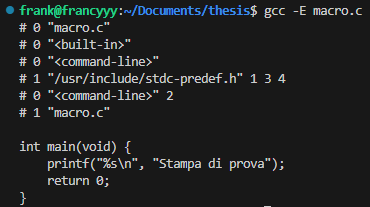
\includegraphics[width=.6\textwidth]{c-macro-preprocess}
        \caption{Traduzione di una \textit{macro} in C}\label{c:macro-preprocess}
    \end{center}
\end{figure}
La natura semplice delle macro C comporta delle limitazioni e falle di sicurezza, molte delle quali sono riportate sulla documentazione GCC\cite{GNU-online-docs}. 
A dimostrazione di ciò, si consideri la seguente modifica del listato~\ref{c:macro}:
\begin{lstlisting}[language=C, caption={Utilizzo scorretto di \textit{macro} in C}, label={c:macro-2}]
#include <stdio.h>
#define printline(x) printf("%s\n", x)
int main(void) {
    int my_val = 150;
    printline(my_val);
    return 0;
}
\end{lstlisting}
Nel listato~\ref{c:macro-2} si tenta di sfruttare la stessa macro, \texttt{printline}, per stampare il contenuto di un intero. 
È interessante osservare che, nonostante il mismatch dei tipi (\texttt{\%s} indica di interpretare il parametro come stringa), il compilatore
 genera soltanto un warning, producendo lo stesso un file eseguibile. 
Tuttavia, tentando l'esecuzione si verifica un crash immediato dovuto a \textit{segmentation fault},
come è osservabile dall'immagine~\ref{c:macro-exec}. \hfill
\begin{figure}[htbp]
    \begin{center}
        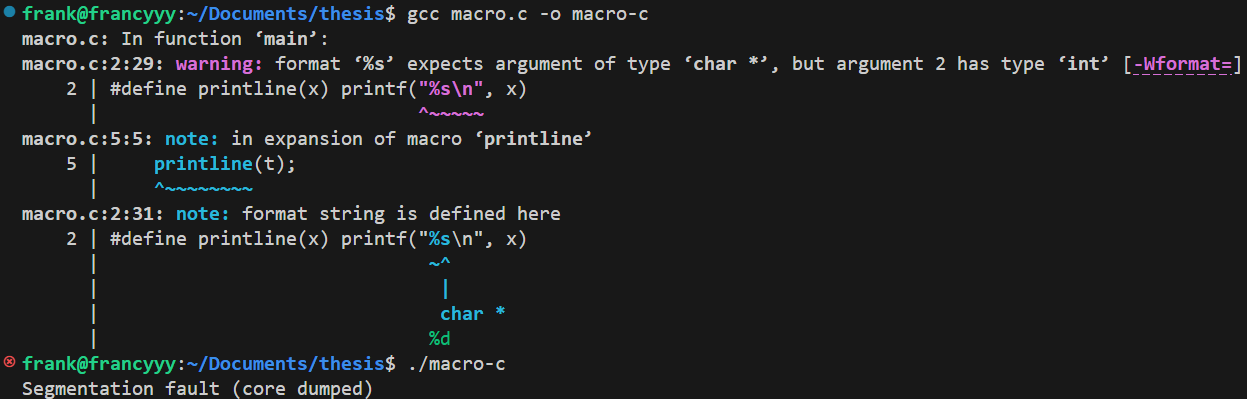
\includegraphics[width=1\textwidth]{c-macro-exec}
        \caption{Limitazioni delle \textit{macro} C}\label{c:macro-exec}
    \end{center}
\end{figure}
\vspace{10pt}\\
\noindent In Rust le \textit{macro} si distinguono in due classi: dichiarative e procedurali. Le \textit{macro} procedurali sono molto complesse e richiederebbero un capitolo
a parte, ma andrebbe oltre l'ambito di questa trattazione. 

Le \textit{macro} dichiarative, pur essendo meno complesse rispetto a quelle procedurali, sono caratterizzate comunque da una sintassi particolare,
basata su \textit{match di pattern}, permettendo
perfino l'\textit{overloading} in base al \textit{pattern} come riportato dalla documentazione ufficiale\cite{rust-book}. 
Anche queste richiederebbero un capitolo 
dedicato per una spiegazione sufficientemente dettagliata. \hfill
\vspace{9pt}\\
\noindent Per mostrare la maggiore complessità, e differente gestione, delle \textit{macro} Rust rispetto alla controparte C, è sufficiente un esempio rappresentativo\footnote{L'esempio fornito è basato su quello riportato nella documentazione ufficiale\cite{rust-book}, nella pagina relativa all'overloading di macro.}:
\begin{lstlisting}[language=Rust, caption={Definizione di \textit{macro} dichiarativa in Rust}, label={rust:macro}]
macro_rules! comp_eval {
    ($sx:expr; and $dx:expr) => {
        println!(
            "{:?} and {:?} is {:?}",
            stringify!($sx), stringify!($dx), $sx && $dx
        )
    };
    ($sx:expr; or $dx:expr) => {
        println!(
            "{:?} or {:?} is {:?}",
            stringify!($sx), stringify!($dx), $sx || $dx
        )
    };
    ($not:expr) => {
        println!(
            "not {:?} is {:?}",
            stringify!($not), !($not)
        )
    };
}
fn main() {
    comp_eval!(1 + 2 == 3; and true);
    comp_eval!(true; or false);
    comp_eval!(true);
}
\end{lstlisting}
Nel listato~\ref{rust:macro} è definita la \textit{macro} dichiarativa \texttt{comp\_eval} che, in base al pattern, espande un codice diverso:
\begin{itemize}
    \item Se viene fornita una coppia di espressioni, \texttt{\$sx} e \texttt{\$dx}, separate dalla parola chiave \texttt{and}, la \textit{macro} espande una stampa della loro congiunzione logica;
    \item Se le espressioni sono separate dalla parola chiave \texttt{or}, espande una stampa della loro disgiunzione logica;
    \item Se invece viene fornita una singola espressione, \texttt{\$not}, la \textit{macro} espande una stampa della sua negazione logica.
\end{itemize}
Il risultato dell'esecuzione di questo codice è osservabile nell'immagine~\ref{rust:correct-macro}. \hfill
\vspace{0pt}\\
\noindent Le \textit{macro} Rust rappresentano uno strumento molto potente rispetto alle direttive pre-processore di C:\  permettono di definire comportamenti 
differenti in base alla struttura dell'invocazione, cosa non
possibile con la semplice sostituzione testuale.

Un'altra differenza rispetto alle \textit{macro} C riguarda la loro espansione: le \textit{macro} in Rust vengono espanse a livello di compilazione e in caso di mancata
corrispondenza con qualsiasi \textit{pattern} previsto viene generato un errore di compilazione.

Ad esempio, aggiungendo l'invocazione `\texttt{comp\_eval!("test")}' all'interno della funzione \texttt{main} nel listato~\ref{rust:macro}, si otterrà un errore
durante la compilazione in quanto il \texttt{pattern} fornito non corrisponde a nessuna delle regole definite nella macro\footnote{In questo esempio il pattern fornito è una singola stringa, quindi la regola adeguata sarebbe la terza, che accetta un'unica espressione. Tuttavia, l'operatore di negazione logica non può essere applicato a una stringa, di conseguenza il compilatore rifiuta il codice, generando un errore.}.
Il messaggio di errore è osservabile nell'immagine~\ref{rust:incorrect-macro}.
\begin{figure}[htbp]
    \begin{center}
        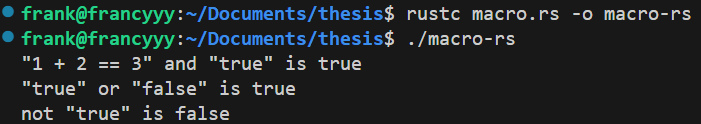
\includegraphics[width=.8\textwidth]{rust-correct-macro}
        \caption{Compilazione di una \textit{macro} in Rust}\label{rust:correct-macro}
    \end{center}
\end{figure}
\begin{figure}[htbp]
    \begin{center}
        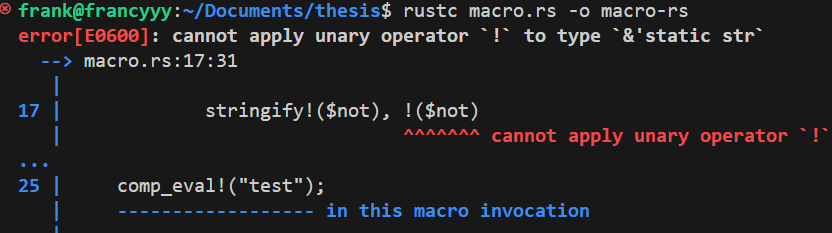
\includegraphics[width=.8\textwidth]{rust-incorrect-macro}
        \caption{Errore durante la compilazione di una \textit{macro} in Rust}\label{rust:incorrect-macro}
    \end{center}
\end{figure}